%===============================================================================
%===============================================================================
%
\clearpage
%
\subsection{Example-0201-u \texttt{[PLAUSIBLE]}}
%
Example uses generated or user-defined regular meshes in CHeart mesh format
and solves a static problem, i.e., applies the boundary conditions in one step.\\[3ex]

Issues/TBD: 2D, iterative solver, analytical Jacobian
%
%===============================================================================
%
\subsubsection{Mathematical model - 3D}
%
We solve the following scalar equation,
%
\begin{align}
    \nabla \cdot \boldsymbol{P} (\boldsymbol{u}, t) = \boldsymbol{0} & &&\Omega = [0, L_X] \times [0, L_Y] \times [0, L_Z],
\end{align}
%
with 1st Piola-Kirchhoff stress tensor in $d$ dimensions,
%
\begin{align}
    \boldsymbol{P} &= \frac{2 \mu}{[\det F]^{2/d}} \left( \boldsymbol{F} - \frac{\boldsymbol{F} : \boldsymbol{F}}{d} \boldsymbol{F}^{-T} \right) - p \boldsymbol{F}^{-T}
\end{align}
%
corresponding to a Neo-Hookean constitutive law (Neo-Hooke parameter $\mu$)
with Dirichlet boundary conditions
%
\begin{align}
    u_x = 0 & &&X = 0, \\
    u_x = u_y = u_z = 0 & && X = Y = Z = 0, \\
		u_x = \lambda * L_X & &&X = L_X.
\end{align}
%
or Dirichlet/Neumann boundary conditions
%
\begin{align}
    u_x = 0 & &&X = 0, \\
    u_x = u_y = u_z = 0 & && X = Y = Z = 0, \\
		\boldsymbol{t} = \begin{bmatrix}
		  \mu (\lambda - \frac{\mu}{\lambda^2}) \\
		  0 \\
		  0
		\end{bmatrix} & &&X = L_X.
\end{align}
%
with stretch $\lambda$ and traction $\boldsymbol{t}$.
%
%===============================================================================
%
\subsubsection{Computational model}
%
\begin{itemize}
    \item{Commandline arguments are:}
        \subitem{float: initial length along x-direction}
        \subitem{float: initial length along y-direction}
        \subitem{float: initial length along z-direction}
        \subitem{integer: number of elements in x-direction}
        \subitem{integer: number of elements in y-direction}
        \subitem{integer: number of elements in z-direction}
        \subitem{integer: use direct solver?}
        \subitem{integer: use finite-difference Jacobian}
        \subitem{float: 1st Mooney-Rivlin parameter}
        \subitem{float: 2nd Mooney-Rivlin parameter (set to zero)}
        \subitem{integer: use generated mesh?}
        \subitem{float: maximum stretch}
        \subitem{integer: use only Dirichlet BC?}
    \item{Commandline arguments for tests are:}
        \subitem{2.0 1.0 1.0  4 2 2 1 1 17.85 0.0 1 0.2 1}
        \subitem{2.0 1.0 1.0  4 2 2 1 1 17.85 0.0 1 0.2 0}
        \subitem{2.0 1.0 1.0  8 4 4 1 1 17.85 0.0 1 0.2 1}
        \subitem{2.0 1.0 1.0  8 4 4 1 1 17.85 0.0 1 0.2 0}
        \subitem{2.0 1.0 1.0 16 8 8 1 1 17.85 0.0 1 0.2 1}
        \subitem{2.0 1.0 1.0 16 8 8 1 1 17.85 0.0 1 0.2 0}
        \subitem{2.0 1.0 1.0  4 2 2 1 1 17.85 0.0 0 0.2 1}
        \subitem{2.0 1.0 1.0  4 2 2 1 1 17.85 0.0 0 0.2 0}
        \subitem{2.0 1.0 1.0  8 4 4 1 1 17.85 0.0 0 0.2 1}
        \subitem{2.0 1.0 1.0  8 4 4 1 1 17.85 0.0 0 0.2 0}
        \subitem{2.0 1.0 1.0 16 8 8 1 1 17.85 0.0 0 0.2 1}
        \subitem{2.0 1.0 1.0 16 8 8 1 1 17.85 0.0 0 0.2 0}
    \item{Note: Binary uses command line arguments to search for the relevant mesh files if user-defined meshes are selected.}
\end{itemize}
%
%===============================================================================
%
\subsubsection{Result summary}
%
We use iron reference results that were compared against an analytical solution.
%
\verbatiminput{examples/example-0201-u/results/results.summary}
\verbatiminput{examples/example-0201-u/results/failed.tests}
%
\begin{figure}[h!]
    \centering 
    \includegraphics[width=0.9\columnwidth]{examples/example-0201-u/doc/figures/iron_reference_3D.eps} 
    \caption{3D results, iron reference w/ command line arguments [...].}
    \label{example-0201-u-iron-3D-reference-fig}
\end{figure}
%
\begin{figure}[h!]
    \centering 
%    \includegraphics[width=0.9\columnwidth]{examples/example-0201-u/doc/figures/current_run_l2x1x1_n8x4x4_i1_s0.eps} 
    \caption{3D results, current run w/ command line arguments [...].}
    \label{example-0201-u-current-run-3D-fig}
\end{figure}
%
%===============================================================================
%===============================================================================
